% ---------------------------------------------------------------------------
% Method (concise). Details live in the appendix files sections/app_*.tex.
% Earlier versions: sections/method_prev*.tex.
% ---------------------------------------------------------------------------
\section{Methodology}
\label{sec:method}

\paragraph{Task.}
\label{sec:task}
Cogniland is a procedurally generated grid world built on OpenSimplex noise
\citep{spencer2014opensimplex}. A successful agent must develop navigation skills and belief integration ability. An episode is one $32\times64$ map crossed from
left to right (Figure~\ref{fig:task}, Appendix~\ref{app:map-generation}). Water
and rock tiles block movement and trees are impassable; the agent can \textsc{build} on the water and \textsc{mine} through rocks.
Each map has a hidden \emph{category} set by its terrain distribution:
\emph{lakes} (more water), \emph{rocky} (more rock) or \emph{balanced}. Every map ends in a narrow passage, followed by a split with two flags signaling terminal states. Only the correct flag pays a terminal reward: the top flag on rocky
maps, the bottom flag on lakes maps, either flag on balanced maps
(Appendix~\ref{app:map-generation}). The agent must form a \textbf{belief}
about the category and carry it across the grass corridor that precedes the passage, while using its
\textbf{skills} to get past the obstacles on the way. Map categories are sampled
uniformly during training.

\begin{figure}[h]
    \centering
    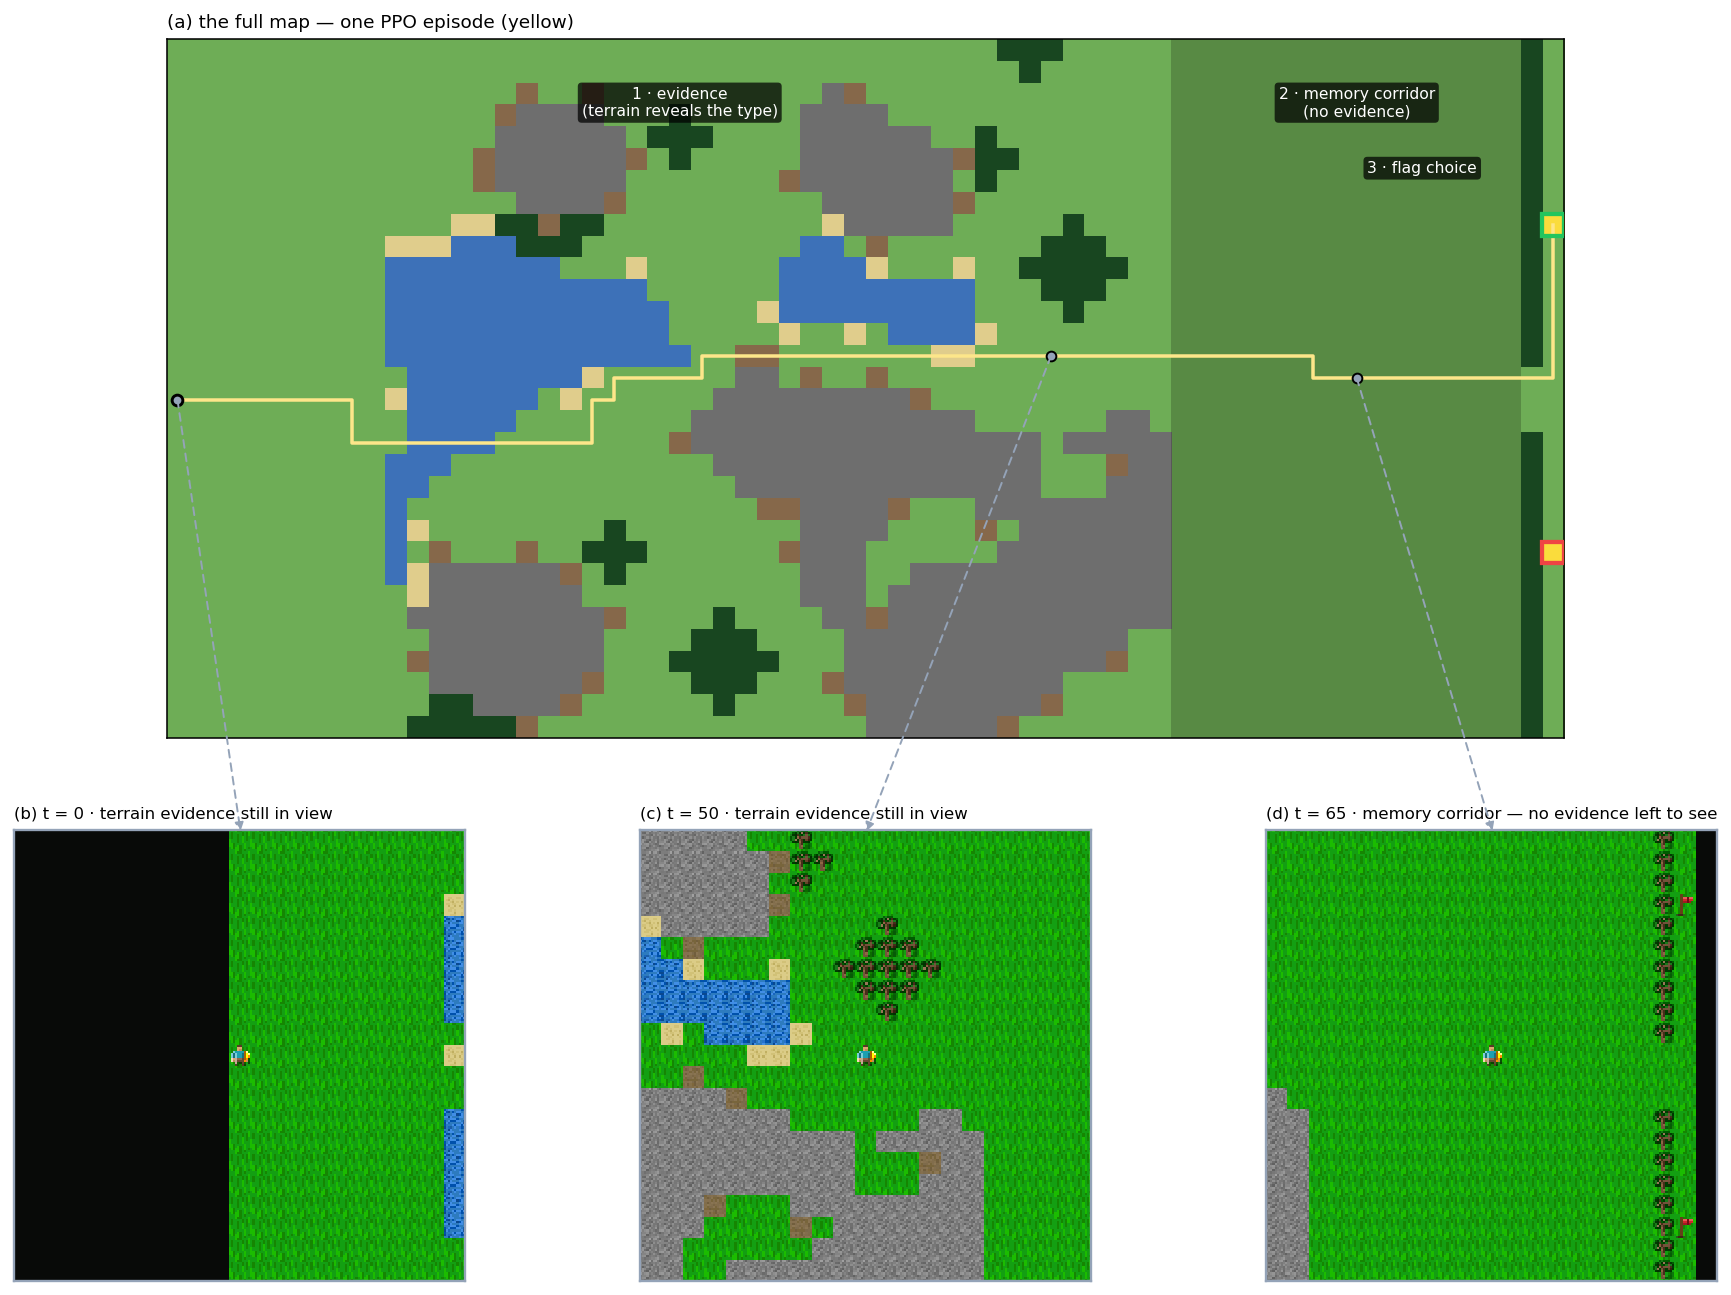
\includegraphics[width=0.6\linewidth]{figures/task.png}
    \caption{\textbf{Anatomy of an episode.} (a) an agent trajectory on a \textit{rocky} map (yellow). Bottom row shows $21\times21$ egocentric observations at different timesteps. (b) The agent starts with little evidence about the map. (c) During the episode the agent navigates obstacles and collects evidence about the map distribution. (d) The agent is presented a choice, only the correct flag returns terminal reward. The choice is determined by the acquired evidence over the episode.}
    \label{fig:task}
\end{figure}

\paragraph{Problem formulation.}
\label{sec:formulation}
The task is a Partially Observable Markov Decision Process (POMDP) with hidden
variable $c\in\{\text{lakes},\text{rocky},\text{balanced}\}$, observations
$o_t$ and actions $a_t$. Three quantities are defined per episode.
\emph{Belief:} $\beta_t = P(c\mid o_{1:t})$, the agent's estimate of which
kind of map it is on. A well-calibrated belief is necessary to achieve high reward: a
Bayes-optimal agent walks to the flag of the most probable category
$\arg\max_c \beta_t(c)$, and on balanced maps either flag is optimal.
The agent carries and updates its belief through the recurrent state
$\mathbf{h}_t$.
\emph{Behavior:} $\phi = (n_{\textsc{build}}, n_{\textsc{mine}})$, the
number of times the agent bridged water and tunnelled rock. Obstacles can be crossed with a tool or walked around (Appendix~\ref{app:measures}).
\emph{Decision:} $D\in\{\text{top},\text{bottom}\}$, the flag the agent
walks into. On lakes and rocky maps one flag pays nothing, so a wrong $D$
shows in the return; on balanced maps both pay, so $D$ is a free choice the
return cannot see.
A steering intervention $\mathcal{I}$ edits the hidden state $\mathbf{h}_t$ to
change the behavior $\phi$, for instance to suppress \textsc{mine} so that the
agent walks around mountains instead. Ideally the intervention $\mathcal{I}$ leaves the belief $\beta$,
and hence the final decision $D$, untouched. We measure \emph{belief corruption} as the change
in the decoded belief and in the final decision $D$ that $\mathcal{I}$ causes.

\paragraph{Model.}
\label{sec:model}
The agent is a recurrent actor-critic policy trained with PPO
\citep{schulman2017ppo} (Figure~\ref{fig:model}): a convolutional encoder of the egocentric view, with
coordinate channels appended \citep{liu2018intriguing}, feeds a GRU \citep{cho2014gru} with $128$-d hidden state $\mathbf{h}_t$. Linear actor
and critic heads read $\pi(a\mid\mathbf{h}_t)$ and the value $V(\mathbf{h}_t)$ from the hidden state. The
training loss is the PPO objective alone; nothing supervises $\mathbf{h}_t$ on
the category, so the belief we decode is emergent (Appendix~\ref{app:model}). Trained on $4{,}800$ maps, the best
agent reaches $98.8\%$ success evaluated on $1{,}200$ held-out maps.

\paragraph{Belief decoding.}
\label{sec:decoding}
Because the belief direction might change over the course of an episode, we split the map's columns into eight position bins, five over the evidence terrain, two over the memory corridor and one at the passage (Appendix~\ref{app:belief-causality}), and fit
and score every readout separately in each bin, evaluating on held-out maps.
In each bin we compare three readouts of $\mathbf{h}_t$: a logistic-regression probe, a one-hidden-layer MLP probe, and a logistic regression on a single scalar, the projection of $\mathbf{h}_t$ on the difference-of-means direction $\mathbf{v}$ between the activations of rocky and lakes maps over a bin. If the belief is linear and one-dimensional, the scalar should match the full-state probes' performance. An episode's belief $\hat b$ is the average projection $b_t=\mathbf{h}_t^{\top}\mathbf{v}$ over bin \textit{corr2}.

\paragraph{Belief causality.}
\label{sec:causality}
A direction may be decodable even if it is not used by the policy \citep{alain2017probes}. To test whether
$\mathbf{v}$ influences the flag decision, we push the state along this direction and leave every other
direction untouched,
$\mathbf{h}'=\mathbf{h}+s\,\alpha\,g\,\mathbf{v}$,
where $g=b^{\star}_{\text{rocky}}-b^{\star}_{\text{lakes}}$ is the distance between
the two category poles, $s=+1$ pushes toward rocky and $s=-1$ toward lakes, and
$\alpha$ is the dose: $\alpha=0$ is the unsteered agent and $\alpha=1$ moves the
belief coordinate by one full pole-to-pole distance. The write is applied once at
the entry of bin \textit{corr2}; lakes maps are pushed toward rocky, rocky maps
toward lakes and balanced maps in both directions, and the outcome is the
decision $D$ as a function of $\alpha$. As a control we apply a displacement of
the same size, $\alpha g$, along random directions.

\paragraph{Steering.}
\label{sec:steering}
Activation steering edits $\mathbf{h}_t$ directly, as popular steering methods
do \citep{turner2023actadd,rimsky2024caa,zou2023repe}. To suppress the skill
associated with an action $\bar a$, here \textsc{build} or \textsc{mine}, we
drive its probability $\pi(\bar a\mid\mathbf{h})$ below a threshold $\theta$ by
gradient steps in activation space:
\begin{equation}
\mathbf{h}\;\leftarrow\;\mathbf{h}-\alpha\,
\frac{\nabla_{\mathbf{h}}\log \pi(\bar a\mid\mathbf{h})}{\lVert\nabla_{\mathbf{h}}\log \pi(\bar a\mid\mathbf{h})\rVert}
\qquad\text{while } \pi(\bar a\mid\mathbf{h})>\theta.
\label{eq:clamp}
\end{equation}
This is applied at every step and carried forward by the recurrence. Steps already
below $\theta$ are left untouched, so $\theta$ sets the strength and $\alpha$
only the step size; a fixed steering vector is the unconditional, one-step
special case (Appendix~\ref{app:steering-algorithm}). Behavior change is the
reduction in successful uses of the suppressed tool relative to the unsteered
agent on the same maps and seeds. We measure the change in belief $\hat b$
and decision $D$ between the steered and unsteered realizations of the policy
(Appendix~\ref{app:measures}).
